\subsubsection{Augmented Reality App}
Augmented Reality er en teknologi der kan sætte virtuelle objekter ind i en virkelig kontekst. Derudover har man mulighed for at interagere med objektet i real tid. 
Denne metode bruger producenten "Artemides" i deres Augmented Reality App. Appen virker ved, at man scanner et logo fra et fysisk lampekatalog, hvorefter en givet lampe vil vise sig på logoets plads. Det er herefter muligt at flytte kataloget for, at se lampen i forskellige kontekster. Derudover har man mulighed for at rotere i alle vinkler samt tænde og slukke for lampens pære. 
Fordelene ved appen er, at brugeren har mulighed for selv at vælge hvilken lampe de vil se i sin egen kontekst, samt interagere med lampen. Herved har brugeren mulighed for, at se præcist hvordan lampen ser ud. 
Ulemperne ved appen er, at den ikke visualisere lampens belysning særlig godt, da dens første priotet er at visualisere selve lampens design. Derudover er det ikke muligt at visualisere lamper i en kontekst, hvis man ikke har den nødvendige bog som indeholder logoer over de forskellige lampedesigns i 3D. En anden ulempe er, at lampeudvalget er meget begrænset da det kun er udvalgte produkter fra "Artemides" som kan visualiseres. 
Nedenstående figur viser "Artemides" brugervejledning til appen.

\begin{figure}[H]
    \centering
    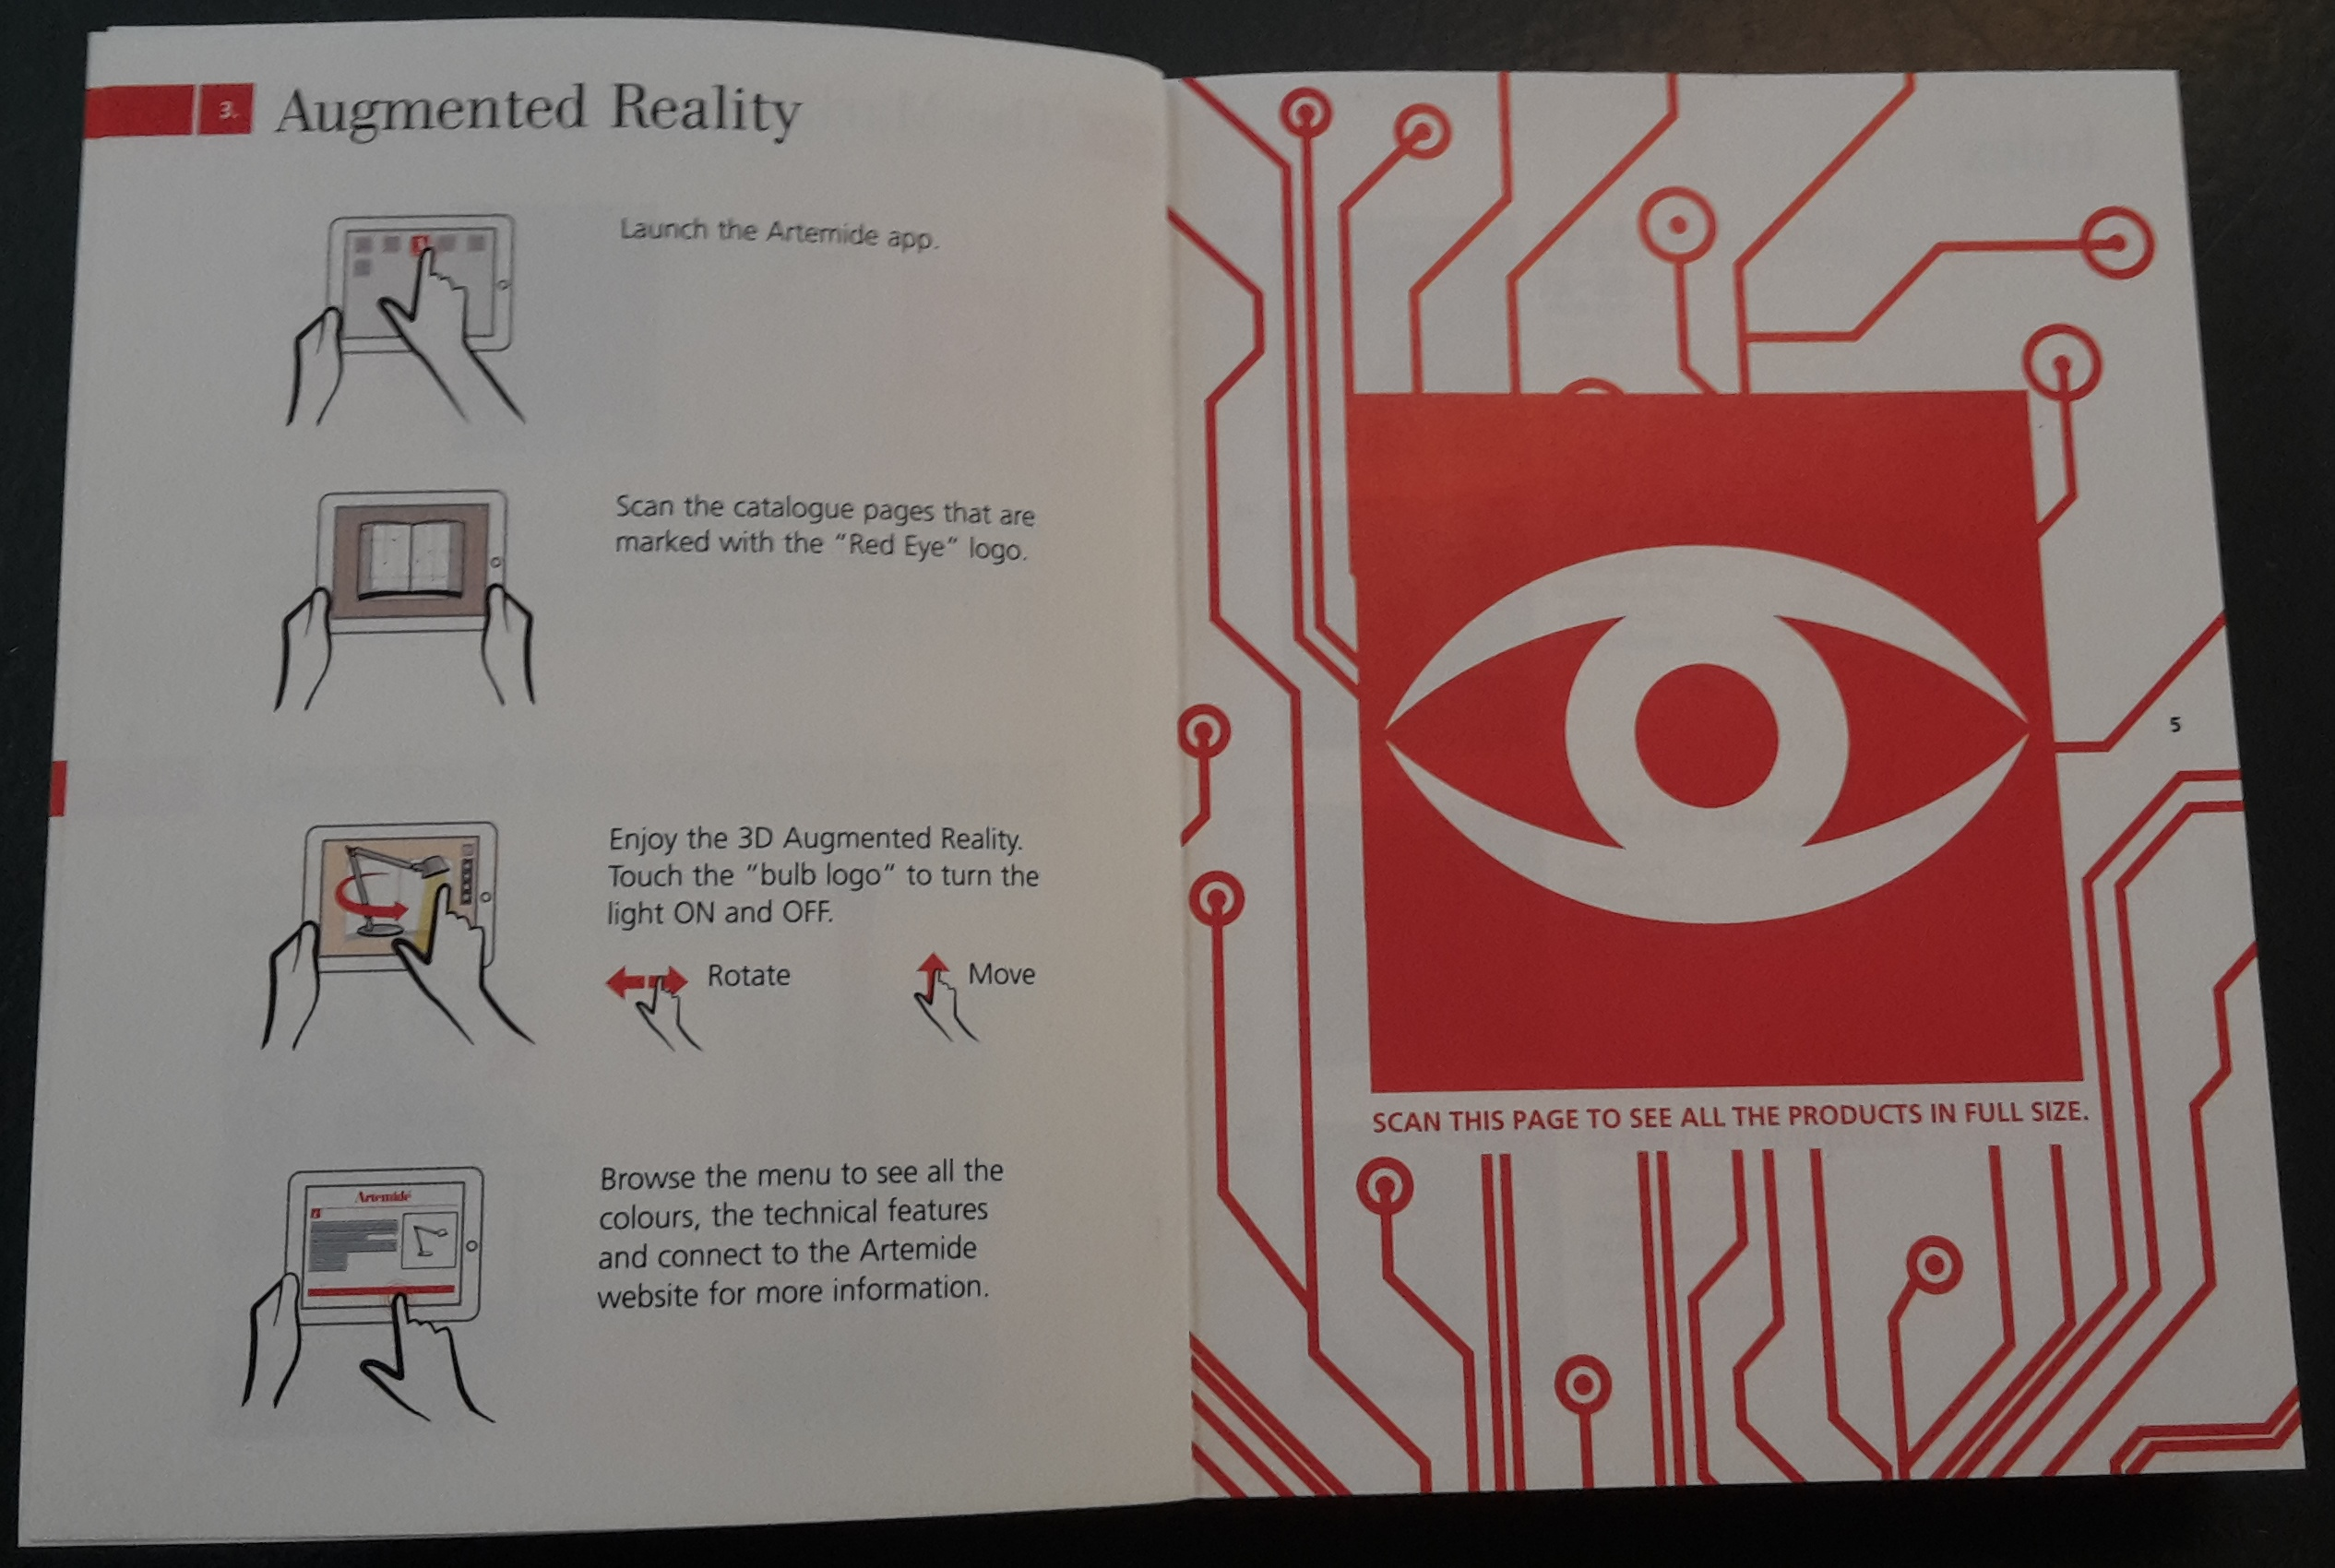
\includegraphics[width=10cm]{augmented_reality_artemides}
    \caption{Brugervejledning fra Artemides augmented reality.}
    \label{fig:augmented_reality_artemides}
\end{figure} 
